\documentclass[12pt,a4paper]{article}
\usepackage[utf8]{inputenc}
\usepackage[T1]{fontenc}
\usepackage{amsmath}
\usepackage{amsfonts}
\usepackage{amssymb}
\usepackage{graphicx}
\usepackage[left=2.54cm, right=2.54cm, top=2.54cm, bottom=2.54cm]{geometry}
\usepackage[hidelinks]{hyperref} %for reference automatically
\usepackage{fancyhdr}

\pagestyle{fancy} % for header and footer
\fancyhf{}
\fancyhead[LE,RO]{Prepared by: Phayuth}
\fancyhead[RE,LO]{Supervisor : Dr.Sarot Srang}
\fancyfoot[LE,RO]{Page \thepage}
\renewcommand{\headrulewidth}{2pt}
\renewcommand{\footrulewidth}{1pt} % for header and footer

% THIS IS THE XML CODE INCLUDE==============================================================
\usepackage{listings}
\usepackage{xcolor}
\definecolor{codegreen}{rgb}{0,0.6,0}
\definecolor{codegray}{rgb}{0.5,0.5,0.5}
\definecolor{codepurple}{rgb}{0.58,0,0.82}
\definecolor{backcolour}{rgb}{0.95,0.95,0.92}
\lstset{
	backgroundcolor=\color{backcolour},   
	commentstyle=\color{codegreen},
	keywordstyle=\color{magenta},
	numberstyle=\tiny\color{codegray},
	stringstyle=\color{codepurple},
	numbers=left,
	breaklines=true,
	tabsize=2,
	basicstyle=\ttfamily\footnotesize,
	literate={\ \ }{{\ }}1
}


\begin{document}
	\section*{\centering Lesson 6 : DC Motor Cascade Control}

	\section{Outer Propositional Velocity and Inner Propositional Integral Torque Control Design }
	\begin{figure}[h]
		\centering
		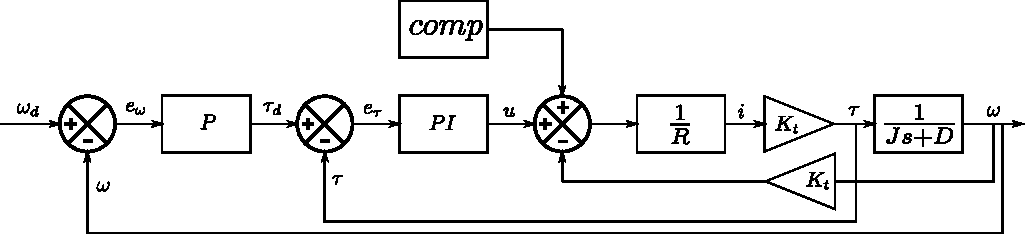
\includegraphics[scale=0.9]{src/img/fig1.pdf}
	\end{figure}

	Assumption: $ L = 0, K_b = K_t, Tc \not= 0$\\
	From the Architecture, We have:
	\begin{itemize}
		\item \(u = K_{pi}e_\tau + K_{ii}\int e_\tau dt + comp\)
		\item \(e_\omega = \omega_d - \omega => \dot{e}_\omega = \dot{\omega}_d - \dot{\omega}\)
		\item \(e_\tau = \tau_d - \tau => \dot{e}_\tau = \dot{\tau}_d - \dot{\tau}\)
		\item \(\tau_d = K_{po}e_\omega => \dot{\tau}_d = K_{po}\dot{e}_\omega\)
	\end{itemize}
	From the Model of DC Model, We have:
	\[
	\begin{split}
		u = K_t\omega + Ri \\
		=> i = \frac{u - K_t\omega}{R}
	\end{split}
	\]
	We have:
	\[
	\tau = K_t i = Tc + D\omega + J\dot{\omega}
	\]
	By Substitute $ i $ in, We get:
	\[
	\begin{split}
		K_t \frac{u - K_t\omega}{R} &= Tc + D\omega + J\dot{\omega} \\
		RT_c + RD\omega + RJ\dot{\omega} &= K_t(u-K_t\omega) \\
		\frac{RJ}{K_t} \dot{\omega} + \frac{RD + K_t^2}{K_t} \omega + \frac{RT_c}{K_t} &= u
	\end{split}
	\]
	Substitute $ u $ in, We get:
	\[
	\begin{split}
		\frac{RJ}{K_t} \dot{\omega} + \frac{RD + K_t^2}{K_t} \omega + \frac{RT_c}{K_t} &= K_{pi}e_\tau + K_{ii}\int e_\tau dt + comp
	\end{split}
	\]
	Take Derivative to eliminate integral:
	\[
	\begin{split}
		\frac{RJ}{K_t} \ddot{\omega} + \frac{RD + K_t^2}{K_t} \dot{\omega} &= K_{pi}\dot{e}_\tau + K_{ii}e_\tau  + \dot{comp}\\
		\frac{RJ}{K_t} \ddot{\omega} + \frac{RD + K_t^2}{K_t} \dot{\omega} &= K_{pi}(\dot{\tau}_d - \dot{\tau}) + K_{ii}(\tau_d - \tau)  + \dot{comp}
	\end{split}
	\]
	From the model, We have:
	\[
	\tau = T_c + D\omega + J\dot{\omega} => \dot{\tau} = D\dot{\omega} + J \ddot{\omega}
	\]
	We get:
	\[
	\begin{split}
		\frac{RJ}{K_t} \ddot{\omega} + \frac{RD + K_t^2}{K_t} \dot{\omega} &= K_{pi}(K_{po}\dot{e}_\omega - (D\dot{\omega} + J \ddot{\omega})) + K_{ii}(K_{po}e_\omega - (T_c + D\omega + J\dot{\omega}))  + \dot{comp} \\	
		\frac{RJ}{K_t} \ddot{\omega} + \frac{RD + K_t^2}{K_t} \dot{\omega} &= K_{pi}(K_{po}\dot{e}_\omega - D\dot{\omega} - J \ddot{\omega}) + K_{ii}(K_{po}e_\omega - T_c - D\omega - J\dot{\omega})  + \dot{comp} \\
		\frac{RJ}{K_t} \ddot{\omega} + \frac{RD + K_t^2}{K_t} \dot{\omega} &= K_{pi}K_{po}\dot{e}_\omega - K_{pi}D\dot{\omega} - K_{pi}J \ddot{\omega} + K_{ii}K_{po}e_\omega - K_{ii}T_c - K_{ii}D\omega - K_{ii}J\dot{\omega}  + \dot{comp} \\
	\end{split}
	\]
	\[
	\begin{split}
		\frac{RJ}{K_t} \ddot{\omega} + \frac{RD + K_t^2}{K_t} \dot{\omega} + K_{pi}D\dot{\omega} + K_{pi}J \ddot{\omega} + K_{ii}D\omega + K_{ii}J\dot{\omega} &= K_{pi}K_{po}\dot{e}_\omega + K_{ii}K_{po}e_\omega - K_{ii}T_c  + \dot{comp} \\
		(\frac{RJ}{K_t} + K_{pi}J ) \ddot{\omega} + (\frac{RD + K_t^2}{K_t}+ K_{pi}D + K_{ii}J) \dot{\omega} + K_{ii}D\omega &=K_{pi}K_{po}\dot{e}_\omega + K_{ii}K_{po}e_\omega - K_{ii}T_c  + \dot{comp}
	\end{split}
	\]
	Multiply both side by -1 to reverse the sign:
	\[
	-(\frac{RJ}{K_t} + K_{pi}J ) \ddot{\omega} - (\frac{RD + K_t^2}{K_t}+ K_{pi}D + K_{ii}J) \dot{\omega} - K_{ii}D\omega = -K_{pi}K_{po}\dot{e}_\omega - K_{ii}K_{po}e_\omega + K_{ii}T_c  - \dot{comp}
	\]
	Adding both of the equation for compensation with :
	\[
	\begin{split}
	&+(\frac{RJ}{K_t} + K_{pi}J ) \ddot{\omega}_d \\
	&+(\frac{RD + K_t^2}{K_t}+ K_{pi}D + K_{ii}J) \dot{\omega}_d \\
	&+K_{ii}D\omega_d
	\end{split}
	\]
	We get:\\
	On LHS:
	\[
	(\frac{RJ}{K_t} + K_{pi}J ) (\ddot{\omega}_d - \ddot{\omega}) + (\frac{RD + K_t^2}{K_t}+ K_{pi}D + K_{ii}J) (\dot{\omega}_d - \dot{\omega})  + K_{ii}D(\omega_d - \omega) = 
	\]
	On RHS:
	\[
	=-K_{pi}K_{po}\dot{e}_\omega - K_{ii}K_{po}e_\omega + K_{ii}T_c  - \dot{comp} +(\frac{RJ}{K_t} + K_{pi}J ) \ddot{\omega}_d + (\frac{RD + K_t^2}{K_t}+ K_{pi}D + K_{ii}J) \dot{\omega}_d+K_{ii}D\omega_d
	\]
	Then:\\
	On LHS:
	\[
	(\frac{RJ}{K_t} + K_{pi}J ) \ddot{e}_\omega + (\frac{RD + K_t^2}{K_t}+ K_{pi}D + K_{ii}J) \dot{e}_\omega  + K_{ii}D e_\omega +K_{pi}K_{po}\dot{e}_\omega + K_{ii}K_{po}e_\omega= 
	\]
	On RHS:
	\[
	= K_{ii}T_c  - \dot{comp} +(\frac{RJ}{K_t} + K_{pi}J ) \ddot{\omega}_d + (\frac{RD + K_t^2}{K_t}+ K_{pi}D + K_{ii}J) \dot{\omega}_d+K_{ii}D\omega_d
	\]
	On LHS:
	\[
	(\frac{RJ}{K_t} + K_{pi}J ) \ddot{e}_\omega + (\frac{RD + K_t^2}{K_t}+ K_{pi}D + K_{ii}J+K_{pi}K_{po}) \dot{e}_\omega + (K_{ii}D+K_{ii}K_{po}) e_\omega = 
	\]
	On RHS:
	\[
	= K_{ii}T_c  - \dot{comp} +(\frac{RJ}{K_t} + K_{pi}J ) \ddot{\omega}_d + (\frac{RD + K_t^2}{K_t}+ K_{pi}D + K_{ii}J) \dot{\omega}_d+K_{ii}D\omega_d
	\]
	On the LHS, Using the 2nd Order Differential Standard Form : $ \ddot{X} + 2\zeta\omega_n\dot{X} + \omega_n^2 X=0 $, We get:
	\[
	2\zeta\omega_n = \frac{(\frac{RD + K_t^2}{K_t}+ K_{pi}D + K_{ii}J+K_{pi}K_{po})}{(\frac{RJ}{K_t} + K_{pi}J )}
	\]
	\[
	\omega_n^2 = \frac{(K_{ii}D+K_{ii}K_{po})}{(\frac{RJ}{K_t} + K_{pi}J )}
	\]
	We solve above equation for $ K_{pi} $ and $ K_{ii} $ in terms of $ K_{po},\zeta,\omega_n $, We get:
	\[
	\begin{split}
		K_{pi} &= -\frac{D^2R+J^2R\omega_n^2+k_{po}(K_t^2-2JR\omega_n\zeta)+D(K_t^2+R(k_{po}-2J\omega_n\zeta))} {K_t(D^2+k_{po}^2+J^2\omega_n^2-2Jk_{po}\omega_n\zeta+2D(k_{po}-J\omega_n\zeta))} \\
		K_{ii} &= \frac{J(-K_t^2+k_{po}R)\omega_n^2} {K_t(D^2+k_{po}^2+J^2\omega_n^2-2Jk_{po}\omega_n\zeta+2D(k_{po}-J\omega_n\zeta))}
	\end{split}
	\]
	On the RHS, We have our compensation:
	\[
	\dot{comp} = K_{ii}T_c +(\frac{RJ}{K_t} + K_{pi}J ) \ddot{\omega}_d + (\frac{RD + K_t^2}{K_t}+ K_{pi}D + K_{ii}J) \dot{\omega}_d+K_{ii}D\omega_d
	\]
	\[
	comp = \int \left[ K_{ii}T_c +(\frac{RJ}{K_t} + K_{pi}J ) \ddot{\omega}_d + (\frac{RD + K_t^2}{K_t}+ K_{pi}D + K_{ii}J) \dot{\omega}_d+K_{ii}D\omega_d\right] dt
	\]
	
\end{document}